\mySection{System Overview}
Our system's primary goal is to help school faculties perform roll calls with ease.
Traditional roll calls usually require teachers to call the names of students one by one
and record students' attendance. Our FRT roll call system will simply take a photo
of the entire classroom and record the attendance of students using Facial Recognition,
thus saving more time for both teachers and students.
\vspace{0.5cm}

Another usage of this system is taking the photo of each student individually as long as
the size of the class is small enough. If the size of the class is too large, this apparently
can result in longer waiting time for the students. Consequently, our main objective is
to ensure that the system can accurately recognize all the faces in a large image
as possible as it can.
\vspace{0.5cm}

We also implement a user-friendly Graphical User Interface (GUI) with PyGTK,
allowing a user (typically a teacher) to perform the following actions:
\vspace{0.5cm}

\setstretch{1}
\begin{enumerate}
  \item Maintain the data of the course and students they teach.
  \item Take photos of students with a camera and train the neural network.
  \item Perform roll calls.
  \item Export the result of roll calls to files.
\end{enumerate}
\setstretch{\myContentLineSpacing}

PyRollCall is able to run on Windows, macOS and unix-like systems as long as
the system has Python3 and X11\footnote{test} installed. All of its external dependencies are already packaged
in the project via Python's \emph{virtualenv}, thus its installation is fairly simple:
\vspace{0.5cm}

\begin{figure}[!htb]
  \centering
  \begin{subfigure}[b]{0.32\linewidth}
    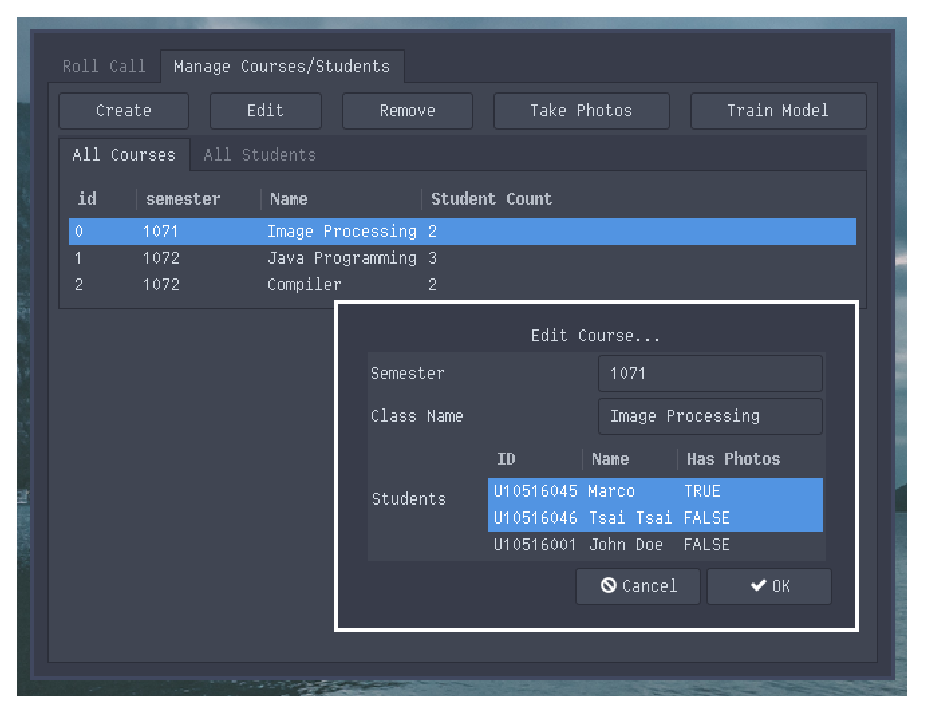
\includegraphics[width=\linewidth]{figures/preview1.eps}
    \caption{Managing courses.}
  \end{subfigure}
  \begin{subfigure}[b]{0.32\linewidth}
    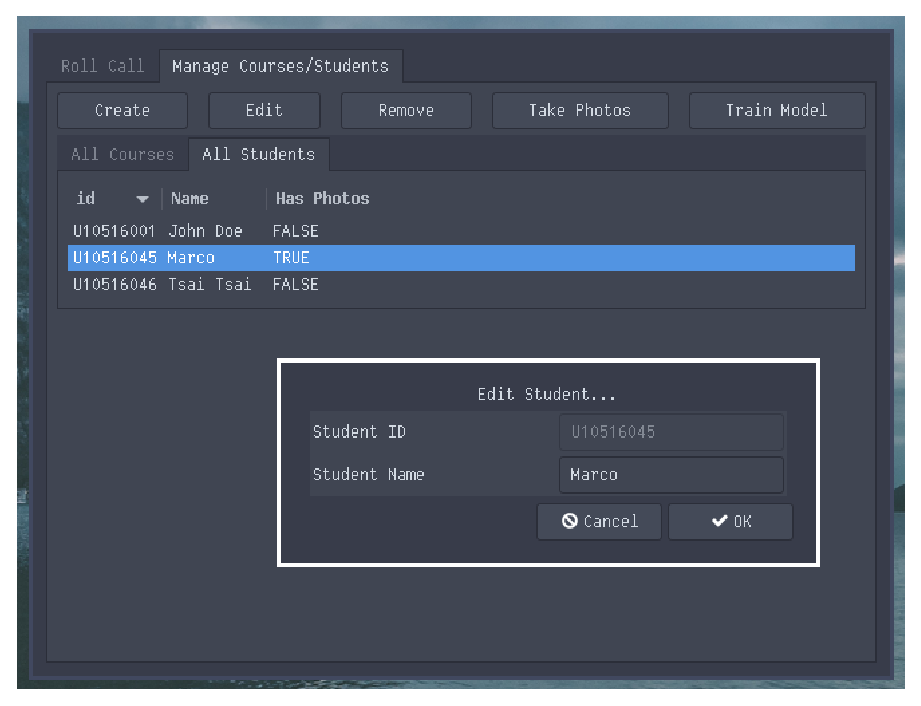
\includegraphics[width=\linewidth]{figures/preview2.eps}
    \caption{Managing students.}
  \end{subfigure}
  \begin{subfigure}[b]{0.32\linewidth}
    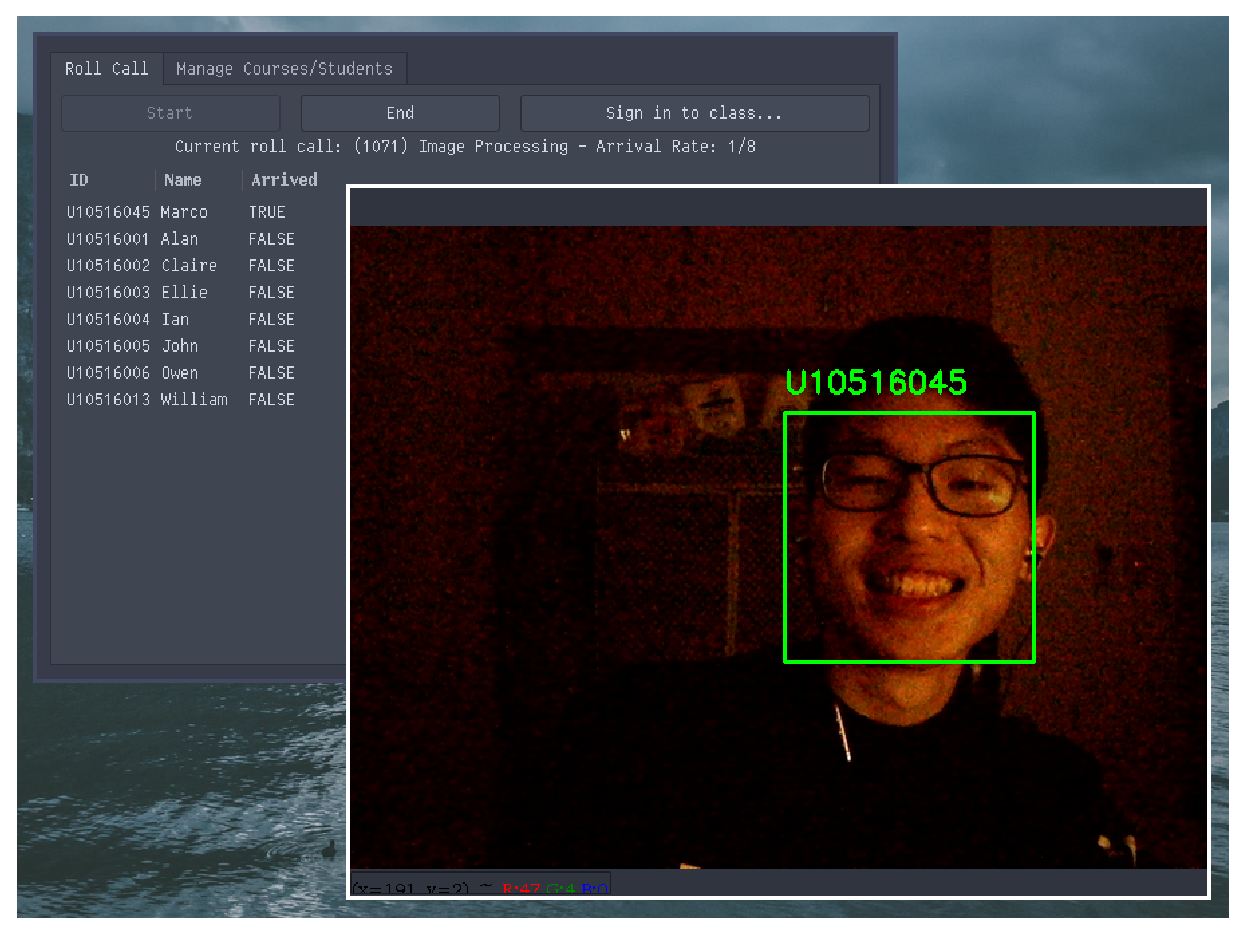
\includegraphics[width=\linewidth]{figures/preview3.eps}
    \caption{A student signing in.}
  \end{subfigure}
  \caption{pyRollCall's GUI, database and facial recognition.}
  \label{fig:implementation}
\end{figure}


\begin{lstlisting}[numbers=none,xleftmargin=0em,caption={Shell commands to checkout and run PyRollCall}]
$ git clone https://github.com/aesophor/pyrollcall.git
$ cd pyrollcall && ./pyrollcall.py 
\end{lstlisting}

By executing \emph{pyrollcall.py}, a Python script located at the project root directory,
users can launch PyRollCall and start using it.

The system comes with an easy-to-use graphical user interface (GUI) crafted with PyGTK,
allowing teachers to easily
(1) Maintain the data of the course and students they teach,
(2) take photos of students via camera,
(3) train the network with the photos of students,
(4) perform roll calls and
(5) export students' attendance to files.

\begin{algorithm}  
\caption{A}  
\label{alg:A}  
\begin{algorithmic}  
\STATE {set $r(t)=x(t)$}   
\REPEAT   
\STATE set $h(t)=r(t)$   
\REPEAT  
\STATE set $h(t)=r(t)$   
\UNTIL{B}   
\UNTIL{B}  
\end{algorithmic}  
\end{algorithm}  
